%%%%%%%%%%%%%%%%%%%%%%%%%%%%%%%%%%%%%%%%%%%%%%%%%%%%%%
%
% $Autor: Srikanth Nanda$
% $Datum: 2020-12-08 11:15:45Z $
% $Pfad: githubtemplate/Template/Presentations/Template/slides/rename.tex $
% $Version: 4620 $
%
% !TeX encoding = utf8
% !TeX root = Rename
%
%%%%%%%%%%%%%%%%%%%%%%%%%%%%%%%%%%%%%%%%%%%%%%%%%%%%

\Mysection{Issac Sim}
\begin{frame}{Overview}
NVIDIA Issac Sim is a robotics simulation platform built on Omniverse for 
photorealistic rendering, GPU-accelerated physics, and high-fidelity sensor simulation 
\cite{NVIDIA:2022}.  
It supports reinforcement learning, motion planning, synthetic data creation, and full-stack 
robotics workflows with Jetson-based robots.  
\end{frame}

\STANDARD{Hardware Requirements for NVIDIA Issac Sim}
{
NVIDIA Issac Sim is a GPU-accelerated robotics simulator built on USD, RTX ray tracing,
and PhysX 5. Therefore, hardware must support real-time ray tracing, high-fidelity physics,
and large-scale scene rendering \cite{HWReq:2024}.
}
\STANDARD{Minimum Requirements (Basic Scenes)}{
\begin{itemize}
    \item \textbf{GPU:} NVIDIA RTX 3060 or Quadro RTX 3000  
    \item \textbf{CUDA Compute Capability:} 7.5+  
    \item \textbf{VRAM:} 6–8 GB  
    \item \textbf{CPU:} Quad-core Intel i5 / AMD Ryzen 5  
    \item \textbf{RAM:} 16 GB  
    \item \textbf{Storage:} 50 GB SSD  
    \item \textbf{OS:} Ubuntu 20.04 / 22.04 or Windows 10/11  
\end{itemize}
}

\STANDARD{Recommended Requirements (Robotics, SLAM, Multi-Robot Scenes)}{
\begin{itemize}
    \item \textbf{GPU:} NVIDIA RTX 3080, RTX 4080, or L40 (industrial)  
    \item \textbf{VRAM:} 12–16 GB for heavy textures + synthetic data  
    \item \textbf{CPU:} 8-core Ryzen 7 / Intel i7 or higher  
    \item \textbf{RAM:} 32 GB or more  
    \item \textbf{Storage:} 200 GB NVMe SSD for USD assets + Omniverse cache  
    \item \textbf{Network:} 1 Gbps for Omniverse Nucleus collaboration  
\end{itemize}
}
\STANDARD{High-End Requirements (Photorealistic Ray-Tracing, Digital Twin Workflows)}{
\begin{itemize}
    \item \textbf{GPU:}  
    \begin{itemize}
        \item NVIDIA RTX 4090 for desktop  
        \item NVIDIA A6000/A8000 for workstation  
        \item NVIDIA H100 for datacenter simulation workloads  
    \end{itemize}
    \item \textbf{VRAM:} 24–48 GB  
    \item \textbf{CPU:} 16-core Threadripper / Xeon workstation  
    \item \textbf{RAM:} 64–128 GB for multi-robot + large environment  
\end{itemize}
}
\STANDARD{RAM and Computation Limitations}{
\begin{itemize}
    \item NVIDIA Issac Sim is heavily optimized for \textbf{RTX ray tracing cores}.  
    \item Scenes involving sensors (RGB, depth, IMU, segmentation) significantly increase VRAM usage.  
    \item Large USD worlds require high disk throughput (fast NVMe recommended).  
    \item Running Issac Sim on laptops is supported, but GPU thermals may limit performance.  
\end{itemize}
}


\STANDARD{Installation Steps for NVIDIA Issac Sim}{
\begin{enumerate}
  \item Install NVIDIA Omniverse Launcher \cite{Omniverse:2023}.  
  \item Download NVIDIA Issac Sim from the Launcher.  
  \item Install dependencies:  
    \begin{itemize}
       \item Python 3.8/3.10  
       \item NVIDIA GPU driver + CUDA  
    \end{itemize}
  \item Verify installation using:
\end{enumerate}

\FILE{./isaac-sim.sh}
}


\Mysection{Packages}
\begin{frame}{NVIDIA Issac Sim Packages}
\begin{itemize}
  \item \textbf{Isaac Core API} — simulation control, physics management \cite{IsaacCore:2023}.  
  \item \textbf{Isaac ROS} — bridges ROS/ROS2 with simulated sensors.  
  \item \textbf{Isaac Replicator} — synthetic data and domain randomization.  
  \item \textbf{Isaac Lab} — RL training environments.  
  \item \textbf{Omnigraph} — node-based control pipelines.  
\end{itemize}
\end{frame}


\begin{frame}{Configuration of NVIDIA Issac Sim}
Configuring NVIDIA Issac Sim correctly is essential for accurate robotics simulation, 
real-time performance, and sensor fidelity \cite{Config:2024}.  
The configuration workflow includes:  
\begin{itemize}
    \item Application Settings  
    \item Physics Engine Configuration  
    \item Sensor Settings  
    \item ROS2 Bridge Configuration  
    \item Scene Setup and Environment Parameters  
    \item Performance Optimization  
\end{itemize}
\end{frame}

%%%%%%%%%%%%%%%%%%%%%%%%%%%%%%%%%%%%%%%%%%%%%%%%%%%%%%
\begin{frame}{Application Settings}

\textbf{1. Render Settings:}
\begin{itemize}
    \item RTX Path Tracing or RTX Real-Time  
    \item Anti-aliasing: TAA or FXAA  
    \item Render Resolution (e.g., 1080p for real-time)  
    \item Shadow Quality and Material Sampling  
\end{itemize}

\textbf{2. Simulation Settings:}
\begin{itemize}
    \item Time step: 60 Hz (default) or 120 Hz for high-speed robots  
    \item Substeps: 4–8 for stable wheel-ground contact  
    \item Gravity: -9.81 m/s\(^2\)  
\end{itemize}

\textbf{3. Resource Management:}
\begin{itemize}
    \item Enable USD Asset Caching  
    \item Limit GPU texture memory if required  
\end{itemize}
\end{frame}

%%%%%%%%%%%%%%%%%%%%%%%%%%%%%%%%%%%%%%%%%%%%%%%%%%%%%%
\begin{frame}{Physics Configuration (PhysX 5)}
\textbf{PhysX Settings}
\begin{itemize}
    \item Solver Type: Temporal Gauss-Seidel (TGS)  
    \item Use GPU Dynamics: Recommended for large scenes  
    \item Restitution, friction, damping settings adjusted per robot  
\end{itemize}

\textbf{Wheel Robot Configuration:}
\begin{itemize}
    \item Enable articulations for wheel joints  
    \item Use differential drive or custom motor model  
    \item Set wheel radius + wheelbase for correct odometry  
\end{itemize}

\textbf{Ground Plane Configuration:}
\begin{itemize}
    \item High-friction surfaces for stable wheel traction  
    \item Collision Mesh Resolution: Medium/High  
\end{itemize}

\end{frame}

%%%%%%%%%%%%%%%%%%%%%%%%%%%%%%%%%%%%%%%%%%%%%%%%%%%%%%
\begin{frame}{Sensor Configuration}

\textbf{Camera Configuration:}
\begin{itemize}
    \item Resolution: 640x480 or 1280x720  
    \item Frame rate: 30–60 FPS  
    \item Intrinsic parameters: fx, fy, cx, cy  
    \item Extrinsic alignment to robot frame  
\end{itemize}

\textbf{IMU Configuration (if used):}
\begin{itemize}
    \item Gyroscope + accelerometer bias  
    \item Noise models (Gaussian)  
\end{itemize}

\textbf{Depth or Segmentation Sensors:}
\begin{itemize}
    \item Enable depth clipping  
    \item Adjust max distance (5–20 m)  
\end{itemize}

\end{frame}

%%%%%%%%%%%%%%%%%%%%%%%%%%%%%%%%%%%%%%%%%%%%%%%%%%%%%%
\begin{frame}{ROS2 Bridge Configuration}

The Isaac ROS2 bridge allows sensor and control topics to flow between 
the robot system and NVIDIA Issac Sim \cite{ROSBridge:2024}.

\textbf{Modules to Enable:}
\begin{itemize}
    \item \PYTHON{/rgb}, \PYTHON{/camera\_info}  
    \item \PYTHON{/cmd\_vel} (Twist)  
    \item \PYTHON{/odom} (Odometry)  
    \item \PYTHON{/tf} and \PYTHON{/tf\_static}  
\end{itemize}

\textbf{Example ROS2 Launch:}

\SHELL{ros2 launch isaac\_ros2\_bridge isaac\_sim\_bridge.launch.py}


\textbf{Simulation Time Sync:}
\begin{itemize}
    \item Use \PYTHON{use\_sim\_time:=true}  
    \item Enable ROS clock publishing  
\end{itemize}

\end{frame}

%%%%%%%%%%%%%%%%%%%%%%%%%%%%%%%%%%%%%%%%%%%%%%%%%%%%%%
\begin{frame}{Environment and Scene Configuration}

\textbf{Scene Composition:}
\begin{itemize}
    \item Load USD environment (warehouse, room, outdoor)  
    \item Insert obstacles for SLAM feature richness  
    \item Adjust lighting for photorealism or performance  
\end{itemize}

\textbf{Robot Setup:}
\begin{itemize}
    \item Import URDF or USD robot model  
    \item Configure joints, limits, inertia  
    \item Attach sensors to correct robot frames  
\end{itemize}

\textbf{Navigation Environment:}
\begin{itemize}
    \item Add ArUco markers (optional)  
    \item Ensure textured surfaces for VSLAM  
\end{itemize}

\end{frame}

%%%%%%%%%%%%%%%%%%%%%%%%%%%%%%%%%%%%%%%%%%%%%%%%%%%%%%
\begin{frame}{Performance Optimization}

\textbf{Real-Time Simulation Tips:}
\begin{itemize}
    \item Lower render resolution (720p for speed)  
    \item Reduce light bounces in path tracing  
    \item Use RTX Real-Time instead of Path Tracing  
    \item Disable unnecessary physics bodies  
\end{itemize}

\textbf{Memory Optimization:}
\begin{itemize}
    \item Reduce texture resolution of non-important assets  
    \item Use instancing when duplicating objects  
\end{itemize}

\textbf{GPU Optimization:}
\begin{itemize}
    \item Enable DLSS (if available)  
    \item Limit simulation to 60 FPS max  
\end{itemize}

\end{frame}

\begin{frame}{Simulated Environment Images}

\begin{figure}[h]
\centering
\includegraphics[width=0.6\textwidth]{example-image}
\caption{Example robot scene rendered in NVIDIA Issac Sim \cite{Render:2024}.}
\end{figure}

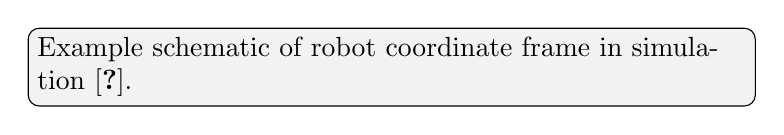
\begin{tikzpicture}
\node[draw,rounded corners,fill=gray!10,text width=9cm]{
Example schematic of robot coordinate frame in simulation \cite{Tikz:2024}.
};
\end{tikzpicture}

\end{frame}

%%%%%%%%%%%%%%%%%%%%%%%%%%%%%%%%%%%%%%%%%%%%%%%%%%%%%%
\Mysection{Localization Slides}
%%%%%%%%%%%%%%%%%%%%%%%%%%%%%%%%%%%%%%%%%%%%%%%%%%%%%%

\begin{frame}{Robot Hardware Used}
\begin{itemize}
  \item NVIDIA Jetson Nano 4GB A02 \cite{Jetson:2020}.  
  \item Raspberry Pi Camera V2 8MP \cite{RPICam:2018}.  
  \item 2-Wheel 48:1 Dagu robot chassis + metal caster \cite{Dagu:2019}.  
  \item ROS2 Humble or Foxy for communication.  
\end{itemize}
\end{frame}

%%%%%%%%%%%%%%%%%%%%%%%%%%%%%%%%%%%%%%%%%%%%%%%%%%%%%%
\begin{frame}{Why No LiDAR?}
Localization is performed using only camera-based visual odometry and wheel-encoder fusion 
instead of LiDAR SLAM \cite{VIO:2022}.  
Advantages:
\begin{itemize}
  \item Lower cost hardware  
  \item Compatible with Jetson Nano  
  \item Works well with Issac Sim synthetic camera feeds  
\end{itemize}
\end{frame}

%%%%%%%%%%%%%%%%%%%%%%%%%%%%%%%%%%%%%%%%%%%%%%%%%%%%%%
\begin{frame}{Camera-Based Localization Pipeline}
\begin{enumerate}
  \item Raspberry Pi V2 Camera simulated in NVIDIA Issac Sim.  
  \item Visual Odometry nodes (Isaac ROS VSLAM).  
  \item Wheel odometry from motor encoders.  
  \item Fusion via Extended Kalman Filter (EKF).  
\end{enumerate}

\begin{figure}
\centering
\includegraphics[width=0.7\textwidth]{example-image-a}
\caption{Visual SLAM pipeline using synthetic camera data in NVIDIA Issac Sim \cite{VSLAM:2023}.}
\end{figure}

\end{frame}

%%%%%%%%%%%%%%%%%%%%%%%%%%%%%%%%%%%%%%%%%%%%%%%%%%%%%%
\begin{frame}[allowframebreaks]{Simulation Setup in NVIDIA Issac Sim}

\textbf{Robot Modeling:}
\begin{itemize}
  \item Import URDF of 2-Wheel Dagu robot.  
  \item Add camera prim at correct height + orientation.  
  \item Configure differential drive controller.  
\end{itemize}

\textbf{Sensor Setup:}
\begin{itemize}
  \item Enable RGB camera + depth (if needed).  
  \item Configure ROS2 bridge topics.  
\end{itemize}

\textbf{Environment:}
\begin{itemize}
  \item Indoor warehouse world.  
  \item Add textures + obstacles for SLAM features.  
\end{itemize}

\framebreak

\textbf{Testing Localization:}

\SHELL{
ros2 launch isaac\_ros\_visual\_slam isaac\_ros\_visual\_slam.launch.py \
    rectified:=true use\_sim\_time:=true}

\end{frame}
